\section{Simulation}
Both the yaw and pitch model serve as a good approximation of force, but they do not adequatley capture the full dynamics of the EndoWrist.
As mentioned in section \ref{se:est}, having a better description of the general dynamics would allow for state estimates useable for state feedback control \cite{yue2004state}.

State feedback control would allow us to control the force output by the EndoWrist without having the ability to measure it during operation.
Estimated states can be used to calculate the force being applied.
Even though the current models do not allow for useable state estimates of the EndoWrist, in this section the opposite is assumed and simulated on the yaw force model.

As seen in ... our simulation model assumes that the EndoWrist yaw force dynamics consist of the linear system and input nonlinearities identified in chapter \ref{ch:fem}.
Our hypothesis is that full reference following capability can be added to the nonlinear system using only position error measurements and the linear model as part of a Kalman filter.

\begin{figure}[H]
\centering
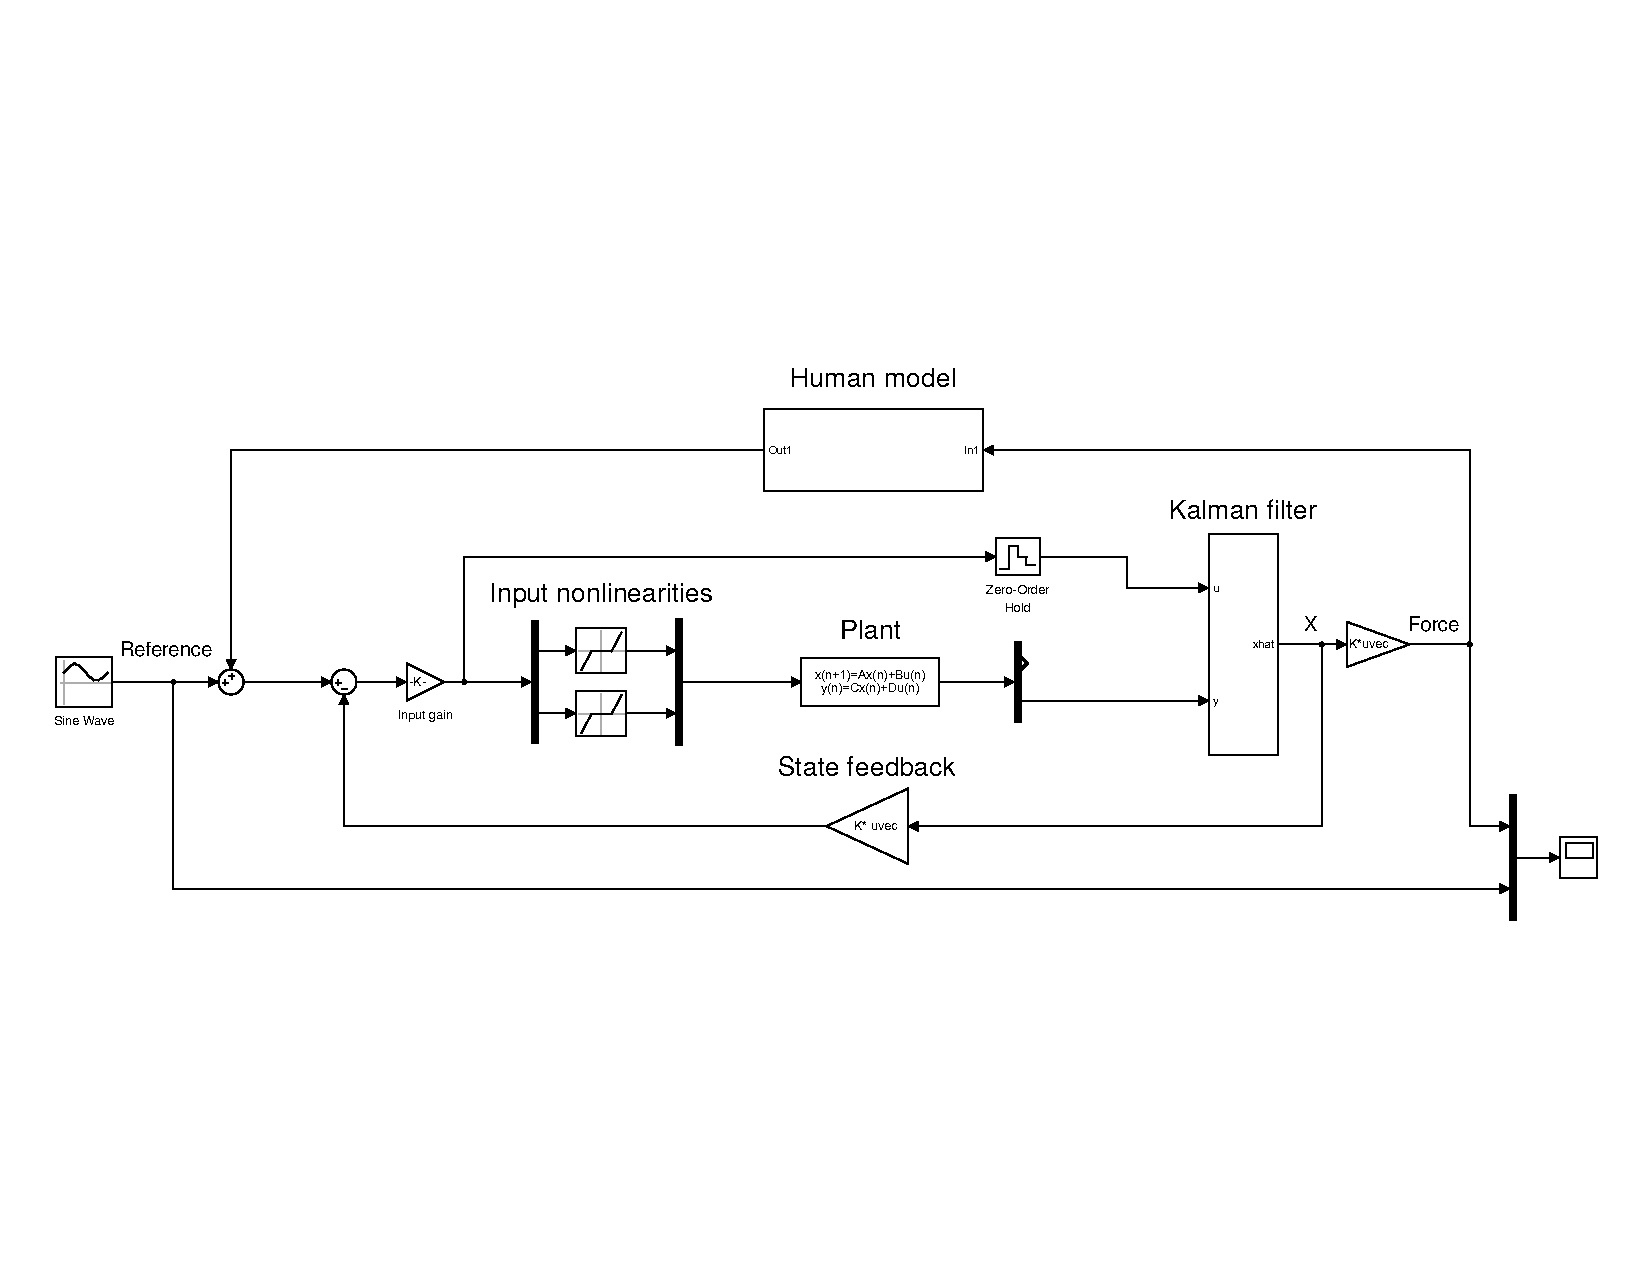
\includegraphics[width=\textwidth]{simsim.pdf}
\caption{Simulation setup.}
\label{figlowpass}
\end{figure}